% Provenance (never printed): old seconde/premiere S material on water as a
% resource (stocks and flows of the water cycle, residence times, groundwater,
% overuse as a physical fact); see sources/book2/PROVENANCE.md. Residence
% times are computed in figdata/grade-10/residence_times.py, the Aral Sea
% budget in figdata/grade-10/aral_sea.py.
\chapter{Les ressources en eau douce}\label{ch:g10:freshwater-resources}

En 1960, la mer d'Aral, dans les déserts d'Asie centrale, était le
quatrième plus grand lac du monde. Deux grands fleuves, alimentés par la
neige et la pluie de montagnes lointaines, s'y jetaient~; aucun n'en
sortait. Dans les années 1960, leur eau fut détournée pour irriguer le
désert. Les satellites ont observé la suite~: le lac s'est morcelé, et la
plus grande partie de son fond est aujourd'hui une terre sèche. La cause, de
très loin, n'a pas été un changement de climat mais l'irrigation~: le lac
recevait chaque année bien moins d'eau que l'évaporation ne lui en
prenait. Ce chapitre fait le compte de l'eau de la Terre, là où elle est
stockée et à quelle vitesse elle circule, et montre qu'une ressource en eau
est avant tout un \omterm{def:g10:freshwater-resources:stock}{flux}~: quand on prélève dans un réservoir plus qu'il n'y
entre, le réservoir se vide, à un rythme que prévoit un simple bilan.
% ledger: nasa:aral, gaybullaev:aral-1960, micklin:aral

\begin{omfigure}
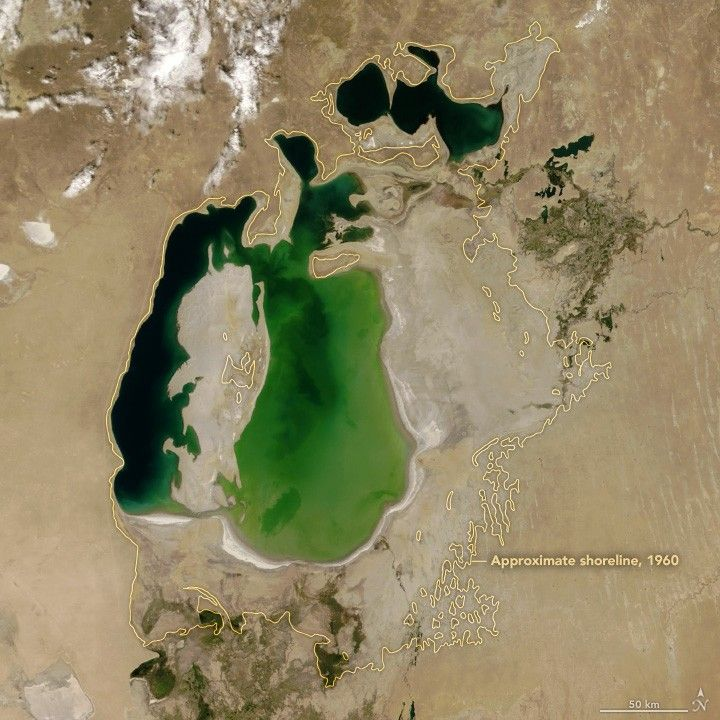
\includegraphics[width=0.47\linewidth]{images/book2/g10-nasa-aral-2000.jpg}\hspace{0.03\linewidth}%
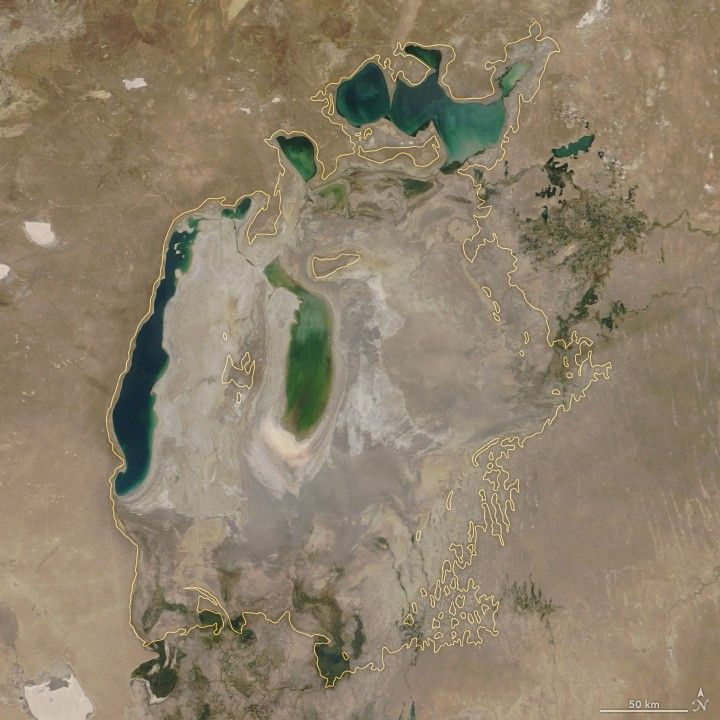
\includegraphics[width=0.47\linewidth]{images/book2/g10-nasa-aral-2018.jpg}

{\small La mer d'Aral vue par l'instrument MODIS du satellite Terra de la
NASA en août 2000 (à gauche) et en août 2018 (à droite)~; la ligne jaune
marque le rivage approximatif de 1960. La barre d'échelle mesure
\qty{50}{km}. Images~: NASA Earth Observatory.}
\end{omfigure}

\begin{recall}
Le cycle de l'eau fait circuler l'eau entre l'océan, l'air et les terres~:
évaporation, condensation en nuages, précipitations, ruissellement~; la
masse totale d'eau se conserve (les livres de physique). Les roches dont
les pores communiquent sont perméables~; sous la surface de la nappe, leurs
pores sont pleins d'eau, et une couche qui contient et laisse passer assez
d'eau pour alimenter des puits est un aquifère (livre~1, année~6). La plus
grande partie de l'eau de la Terre est salée (livre~1, année~2). Une
rivière évacue l'eau de son \omterm{def:g10:drainage-basins:drainage-basin}{bassin versant}~; son \omterm{def:g10:drainage-basins:discharge}{débit} est un volume par
seconde (\cref{ch:g10:drainage-basins}).
\end{recall}

\section{Où se trouve l'eau}

La Terre contient environ 1.39~milliard de kilomètres cubes d'eau. Presque
toute cette eau se trouve dans l'océan~; \qty{2.5}{\percent} seulement est
douce. Et la plus grande partie de cette eau douce est hors d'atteinte~:
plus des deux tiers sont gelés dans les calottes glaciaires et les
glaciers, et près d'un tiers se trouve sous terre.
% ledger: usgs:water-stocks

\begin{center}
\small
\begin{tabular}{|l|r|r|}
\hline
\textbf{réservoir} & \textbf{volume (\unit{km^3})} & \textbf{part de l'eau douce} \\ \hline
océans, mers et baies & \num{1338000000} & (salée) \\ \hline
calottes, glaciers et neiges permanentes & \num{24064000} & \qty{68.7}{\percent} \\ \hline
eaux souterraines douces & \num{10530000} & \qty{30.1}{\percent} \\ \hline
glace du sol et pergélisol & \num{300000} & \qty{0.86}{\percent} \\ \hline
lacs d'eau douce & \num{91000} & \qty{0.26}{\percent} \\ \hline
humidité du sol & \num{16500} & \qty{0.05}{\percent} \\ \hline
atmosphère & \num{12900} & \qty{0.04}{\percent} \\ \hline
rivières & \num{2120} & \qty{0.006}{\percent} \\ \hline
\end{tabular}

{\small Une estimation de l'eau du monde, d'après Shiklomanov (1993), citée
par l'U.S. Geological Survey. Les eaux souterraines salées
(\num{12870000}~\unit{km^3}) et les lacs salés ne sont pas comptés.}
\end{center}
% ledger: usgs:water-stocks

Les rivières et les lacs d'eau douce, où l'on puise la plus grande partie
de l'eau utilisée, contiennent ensemble moins d'un centième de pour cent de
toute l'eau. Pourtant, les rivières ne s'assèchent jamais longtemps~: ce ne
sont pas un \omterm{def:g10:freshwater-resources:stock}{stock} mais un \omterm{def:g10:freshwater-resources:stock}{flux}, renouvelé à chaque pluie.

\section{Stocks et flux}

\begin{definition}[Stock~; flux]\label{def:g10:freshwater-resources:stock}
Dans un bilan d'eau, un \emph{stock}\index{stock (d'eau)} est la quantité
d'eau contenue dans un réservoir --- l'océan, l'air, la glace, un aquifère,
un lac --- à un instant donné, exprimée en volume ou en masse. Un
\emph{flux}\index{flux (d'eau)} est la quantité qui passe d'un réservoir à un autre par unité
de temps, par exemple en kilomètres cubes par an.
\end{definition}

Un \omterm{def:g10:freshwater-resources:stock}{stock} ne change que par ses \omterm{def:g10:freshwater-resources:stock}{flux}~: ce qui entre moins ce qui sort. Quand
les deux sont égaux, le \omterm{def:g10:freshwater-resources:stock}{stock} est en \emph{régime permanent}~: il reste le
même, bien que son eau soit sans cesse remplacée.

\begin{omfigure}
\begin{tikzpicture}[font=\footnotesize, >={Stealth[length=6pt]}]
  % ocean, land, atmosphere
  \fill[omSea] (0,0) rectangle (6.4,1.6);
  \fill[omLithAlluv] (6.4,0) -- (6.4,1.6) -- (8.2,2.1) -- (10.4,2.6) -- (12,2.9) -- (12,0) -- cycle;
  \fill[omLithSand!60] (6.4,0) -- (12,0) -- (12,1.0) -- (6.4,0.7) -- cycle;
  \draw[black!50] (6.4,1.6) -- (8.2,2.1) -- (10.4,2.6) -- (12,2.9);
  \fill[omIce] (10.6,2.65) -- (11.3,3.35) -- (12,2.9) -- cycle;
  \node[align=center] at (3.2,0.75) {\textbf{océan}\\\num{1335040}};
  \node[align=center] at (9.3,1.35) {humidité du sol 122\\lacs et rivières 178};
  \node[align=center] at (9.3,0.35) {eaux souterraines \num{15300}};
  \node[align=center] at (11.2,2.25) {glace\\\num{26350}};
  % atmosphere
  \draw[black!30, rounded corners=8pt, fill=omWxCloud] (1.0,4.6) rectangle (11.0,5.6);
  \node[align=center] at (6.0,5.1) {\textbf{atmosphère} 12.7};
  % fluxes
  \draw[->, omProp, line width=1.4pt] (1.4,1.7) -- node[left, align=right] {évaporation\\413} (1.4,4.5);
  \draw[->, omWxRain, line width=1.4pt] (4.4,4.5) -- node[pos=0.3, right, align=left] {précipitations\\373} (4.4,1.7);
  \draw[->, omWxRain, line width=1.4pt] (7.6,4.5) -- node[pos=0.7, left, align=right] {précipitations\\113} (7.6,2.05);
  \draw[->, omProp, line width=1.4pt] (10.0,2.6) -- node[right, align=left] {évaporation et\\transpiration 73} (10.0,4.5);
  \draw[->, black!60, line width=1.2pt] (4.9,5.85) -- node[above] {vapeur d'eau transportée au-dessus des terres~: 40} (7.4,5.85);
  \draw[->, omRiver, line width=1.4pt] (7.6,1.2) -- node[above, inner sep=2pt] {ruissellement 40} (6.0,1.2);
\end{tikzpicture}

{\small Le cycle global de l'eau des années 1990 (schéma, sans échelle).
\omterm{def:g10:freshwater-resources:stock}{Stocks} en milliers de \unit{km^3}, \omterm{def:g10:freshwater-resources:stock}{flux} en milliers de \unit{km^3} par an.
D'après Trenberth et ses collègues (2007). Les estimations des \omterm{def:g10:freshwater-resources:stock}{stocks}
diffèrent d'une étude à l'autre~: comparer les eaux souterraines et la glace
de ce schéma avec le tableau ci-dessus.}
\end{omfigure}
% ledger: trenberth:water-cycle

Le cycle est équilibré. Chaque année, l'océan perd \num{413000}~\unit{km^3}
par évaporation et en récupère \num{373000} sous forme de pluie et de neige
et \num{40000} par les fleuves. L'air reçoit
$413\,000 + 73\,000 = \num{486000}$~\unit{km^3}
et rend $373\,000 + 113\,000$, soit autant. Les terres reçoivent
\num{113000}~\unit{km^3} de précipitations~; \num{73000} retournent à l'air
par évaporation et par les feuilles des plantes, et les \num{40000} restants
ruissellent jusqu'à la mer, dans les fleuves et sous terre.
% ledger: trenberth:water-cycle

\begin{definition}[Eau douce renouvelable]\label{def:g10:freshwater-resources:renewable}
L'\emph{eau douce renouvelable}\index{eau douce renouvelable} d'une région
est le \omterm{def:g10:freshwater-resources:stock}{flux} d'eau douce renouvelé chaque année par les précipitations, qui
la traverse en ruisselant dans les rivières et sous forme d'eaux
souterraines. C'est un \omterm{def:g10:freshwater-resources:stock}{flux}, en kilomètres cubes par an, et non un \omterm{def:g10:freshwater-resources:stock}{stock}.
\end{definition}

Pour l'ensemble des terres de la Terre, ce sont les \num{40000}~\unit{km^3}
qui atteignent la mer chaque année. Une région peut utiliser son eau
renouvelable année après année sans en manquer. Ce qu'elle prélève au-delà
ne peut venir que d'un \omterm{def:g10:freshwater-resources:stock}{stock}, qui alors diminue.

\section{Le temps de résidence}

Combien de temps une molécule d'eau reste-t-elle dans un réservoir~?
Certaines en sortent aussitôt, d'autres y restent bien plus longtemps~; mais
en moyenne, la réponse découle du seul \omterm{def:g10:freshwater-resources:stock}{stock} et du seul \omterm{def:g10:freshwater-resources:stock}{flux}.

\begin{definition}[Temps de résidence]\label{def:g10:freshwater-resources:residence-time}
Le \emph{temps de résidence}\index{temps de residence@temps de résidence}
de l'eau dans un réservoir est la durée moyenne que l'eau y passe entre son
entrée et sa sortie.
\end{definition}

\begin{proposition}[Temps de résidence, stock et flux]\label{prop:g10:freshwater-resources:residence}
Pour un réservoir en régime permanent, contenant un \omterm{def:g10:freshwater-resources:stock}{stock} $S$ traversé par
un \omterm{def:g10:freshwater-resources:stock}{flux} $F$ (en entrée et en sortie), le \omterm{def:g10:freshwater-resources:residence-time}{temps de résidence} vaut
\[
T = \frac{S}{F}.
\]
\end{proposition}

\begin{proof}
En régime permanent, un volume $F$ entre et un volume $F$ sort chaque année,
tandis que le \omterm{def:g10:freshwater-resources:stock}{stock} reste égal à $S$. Au bout d'une durée $S/F$, un volume $F \times S/F = S$ est
entré~: autant que tout ce que contient le réservoir. En moyenne, l'eau
présente au départ a alors été remplacée, si bien que l'eau reste $S/F$
dans le réservoir.
\end{proof}

\begin{example}[L'eau de l'air]\label{ex:g10:freshwater-resources:atmosphere}
L'atmosphère contient \num{12700}~\unit{km^3} d'eau, et
\num{486000}~\unit{km^3} en tombent chaque année sous forme de pluie et de
neige. Son \omterm{def:g10:freshwater-resources:residence-time}{temps de résidence} vaut $12\,700/486\,000 \approx \num{0.026}$
an, environ \num{9.5}~jours~: l'eau de l'air se renouvelle toutes les une à
deux semaines. Un nuage qui donne de la pluie aujourd'hui est fait d'eau qui
a quitté l'océan ou le sol il y a quelques jours.
\end{example}
% ledger: trenberth:water-cycle (t_atmosphere_days 9.5 in figdata/grade-10/residence_times.py)

Le même calcul donne environ \num{19}~jours pour l'eau des lits des rivières
($2120$~\unit{km^3} parcourus par \num{40000}~\unit{km^3} par an), quelques
années pour les lacs et les rivières ensemble, et environ \num{3200}~ans
pour l'océan ($1\,335\,040/413$ milliers de~\unit{km^3}). Les eaux
souterraines peuvent être plus lentes encore~: l'eau la plus profonde de
certains aquifères est vieille de centaines de milliers d'années.
% ledger: trenberth:water-cycle, usgs:water-stocks, sturchio:nubian-age

\begin{omfigure}
\begin{tikzpicture}
\begin{axis}[omrecord, xbar, xmode=log, log origin=infty, width=0.74\linewidth, height=5.6cm,
  xmin=1, xmax=1e9, ymin=-0.6, ymax=4.6, bar width=11pt,
  ytick={0,1,2,3,4}, yticklabels={atmosphère, rivières, {lacs et rivières}, océan, {eaux souterraines profondes (âge)}},
  xtick={1,30.44,365.25,36525,3652500,365250000}, xticklabels={1 jour, 1 mois, 1 an, 100 ans, \num{10000} ans, 1 million d'années},
  xticklabel style={font=\scriptsize, rotate=25, anchor=north east}, yticklabel style={font=\small},
  xlabel={temps de résidence (échelle logarithmique)}, label style={font=\small}, xmajorgrids]
\addplot[fill=omDef!45, draw=omDef!80!black] table[x=days, y=idx] {figdata/out/grade-10-residence_times-times.dat};
\draw[fill=omProp!45, draw=omProp!80!black] (axis cs:73050000,3.75) rectangle (axis cs:365250000,4.25);
\node[anchor=west, font=\scriptsize] at (axis cs:9.5,0) {\num{9.5}~jours};
\node[anchor=west, font=\scriptsize] at (axis cs:19.4,1) {\num{19}~jours};
\node[anchor=west, font=\scriptsize] at (axis cs:1625,2) {\num{4.5}~ans};
\node[anchor=west, font=\scriptsize] at (axis cs:1180690,3) {\num{3200}~ans};
\node[anchor=east, font=\scriptsize] at (axis cs:73050000,4) {\num{200000} à 1~million d'années};
\end{axis}
\end{tikzpicture}

{\small \omterm{def:g10:freshwater-resources:residence-time}{Temps de résidence} de l'eau, calculés comme le \omterm{def:g10:freshwater-resources:stock}{stock} divisé par le
\omterm{def:g10:freshwater-resources:stock}{flux} à partir du cycle global de l'eau (en bleu), et âge mesuré des eaux
souterraines profondes sous l'est du Sahara (en orange). Axe
logarithmique~: à partir d'un an, chaque graduation marque un facteur cent.
Données~: Trenberth et ses collègues (2007)~; U.S. Geological Survey~;
Sturchio et ses collègues (2004).}
\end{omfigure}
% values computed in figdata/grade-10/residence_times.py

Le \omterm{def:g10:freshwater-resources:residence-time}{temps de résidence} mesure la vitesse à laquelle un réservoir se
reconstitue. L'eau prélevée dans une rivière est remplacée en quelques
jours~; un lac pollué ou vidé demande des années~; des eaux souterraines qui
ont mis des milliers d'années à s'accumuler ne se renouvellent pas du tout
à l'échelle d'une vie humaine.

\begin{method}[Un bilan d'eau]\label{met:g10:freshwater-resources:budget}
\begin{enumerate}
  \item Choisir le réservoir~: un lac, un aquifère, un bassin, l'air.
  \item Dresser la liste de tous les \omterm{def:g10:freshwater-resources:stock}{flux} qui y entrent (rivières, pluie,
        infiltration) et qui en sortent (rivières, évaporation, pompage),
        dans la même unité.
  \item La variation du \omterm{def:g10:freshwater-resources:stock}{stock} par an est la somme des entrées moins la
        somme des sorties.
  \item Si le \omterm{def:g10:freshwater-resources:stock}{stock} ne change pas, les entrées égalent les sorties, et le
        \omterm{def:g10:freshwater-resources:residence-time}{temps de résidence} est le \omterm{def:g10:freshwater-resources:stock}{stock} divisé par l'une ou l'autre.
\end{enumerate}
\end{method}

\section{Les aquifères, des réservoirs}

La pluie qui s'infiltre dans le sol et atteint la surface de la nappe
\emph{recharge} l'aquifère sous-jacent. L'eau circule ensuite lentement
dans les pores de la roche, vers des sources, des rivières ou la mer. Là où
une couche perméable plonge sous une couche imperméable, comme une argile,
son eau est \emph{captive}~: elle n'est alimentée que là où la couche
affleure, ce qui peut être loin.

\begin{omfigure}
\begin{tikzpicture}[font=\footnotesize, >={Stealth[length=5pt]}]
  % layers dipping to the right
  \fill[lith shale] (0,0) -- (12,0) -- (12,0.8) -- (0,2.4) -- cycle;
  \fill[lith sandstone] (0,2.4) -- (12,0.8) -- (12,2.2) -- (2.2,3.5) -- (0,3.8) -- cycle;
  \fill[lith shale] (2.2,3.5) -- (12,2.2) -- (12,3.4) -- (3.6,3.9) -- cycle;
  % ground surface
  \draw[line width=0.8pt, brown!60!black] (0,3.8) -- (1.2,4.0) -- (2.2,3.9) -- (3.6,3.9) -- (6,3.6) -- (9,3.5) -- (12,3.4);
  \fill[omLithAlluv] (0,3.8) -- (1.2,4.0) -- (2.2,3.9) -- (2.2,3.5) -- (0,3.8) -- cycle;
  \fill[omLithAlluv] (2.2,3.9) -- (3.6,3.9) -- (2.2,3.5) -- cycle;
  \fill[omLithAlluv] (3.6,3.9) -- (6,3.6) -- (9,3.5) -- (12,3.4) -- (3.6,3.9) -- cycle;
  % water table in the unconfined part
  \draw[omDef, line width=1pt, dashed] (0,3.3) .. controls (1.0,3.35) and (1.8,3.2) .. (2.6,3.45);
  \node[anchor=south west, text=omDef, fill=white, fill opacity=0.8, text opacity=1, inner sep=1pt] at (0.05,2.75) {surface de la nappe};
  % rain and recharge
  \foreach \x in {0.35,0.65,0.95,1.25} \draw[omWxRain, thick] (\x,4.9) -- (\x-0.15,4.4);
  \node[anchor=south, text=omWxRain] at (0.7,4.95) {pluie~: recharge};
  % flow arrows in the aquifer
  \draw[->, omDef, line width=1.1pt] (2.0,2.85) -- (4.4,2.55);
  \draw[->, omDef, line width=1.1pt] (5.4,2.4) -- (7.8,2.1);
  \draw[->, omDef, line width=1.1pt] (8.8,1.95) -- (11.2,1.65);
  % wells
  \draw[black!70, line width=1.6pt] (1.95,3.95) -- (1.95,2.9);
  \node[anchor=south] at (1.95,4.0) {puits};
  \draw[black!70, line width=1.6pt] (7.0,3.55) -- (7.0,1.9);
  \node[anchor=south] at (7.0,3.6) {puits};
  % labels
  \node[align=center, fill=white, fill opacity=0.85, text opacity=1, inner sep=1.5pt] at (1.5,0.8) {argile imperméable};
  \node[align=center, fill=white, fill opacity=0.85, text opacity=1, inner sep=1.5pt] at (8.6,2.95) {argile imperméable};
  \node[anchor=north, align=center] at (1.6,-0.1) {nappe libre~:\\zone de recharge};
  \node[anchor=north, align=center] at (6.4,-0.1) {nappe captive};
  \node[anchor=north, align=center] at (10.6,-0.1) {eau ancienne, loin de\\la zone de recharge};
\end{tikzpicture}

{\small Un aquifère dans un grès perméable (schéma). La pluie le recharge là
où il affleure~; la surface de la nappe y est libre de monter et de
descendre. Plus loin, sous l'argile, l'aquifère est captif, et son eau
descend lentement le long de la couche~: plus on s'éloigne de la zone de
recharge, plus l'eau est ancienne.}
\end{omfigure}

\begin{definition}[Eau souterraine fossile]\label{def:g10:freshwater-resources:fossil-groundwater}
Une \emph{eau souterraine fossile}\index{eau souterraine fossile} est une
eau souterraine entrée dans son aquifère il y a longtemps, souvent sous un
climat plus humide, et que la recharge actuelle ne renouvelle pas à
l'échelle des vies humaines.
\end{definition}

Sous l'est du Sahara s'étend un vaste aquifère gréseux. Son eau la plus
profonde, datée par la désintégration d'une forme radioactive rare du
krypton, est vieille de \num{200000} à un million d'années. Elle s'y est
écoulée lentement depuis une zone de recharge située dans le sud-ouest de
l'Égypte, et sa chimie montre qu'elle est tombée en pluie lors de périodes
humides passées des âges glaciaires, quand l'air humide venu de
l'Atlantique atteignait la région. Pompée aujourd'hui, une telle eau est un
\omterm{def:g10:freshwater-resources:stock}{stock} que l'on exploite comme une mine, et non un \omterm{def:g10:freshwater-resources:stock}{flux}.
% ledger: sturchio:nubian-age

Quand le pompage dépasse la recharge, la surface de la nappe baisse. Dans
les Hautes Plaines du centre des États-Unis, l'aquifère situé sous quelque
\num{175000}~milles carrés (\qty{453000}{km^2}) est pompé pour l'irrigation
depuis 1950 environ. En 2015, son niveau d'eau avait baissé de \qty{4.8}{m}
en moyenne, et jusqu'à \qty{71}{m} (234~pieds) dans certains puits~;
l'aquifère avait perdu environ \num{273}~millions d'acres-pieds d'eau, soit
quelque \qty{340}{km^3}.
% ledger: mcguire:high-plains (1 acre-foot = 1233.5 m3)

\begin{omfigure}
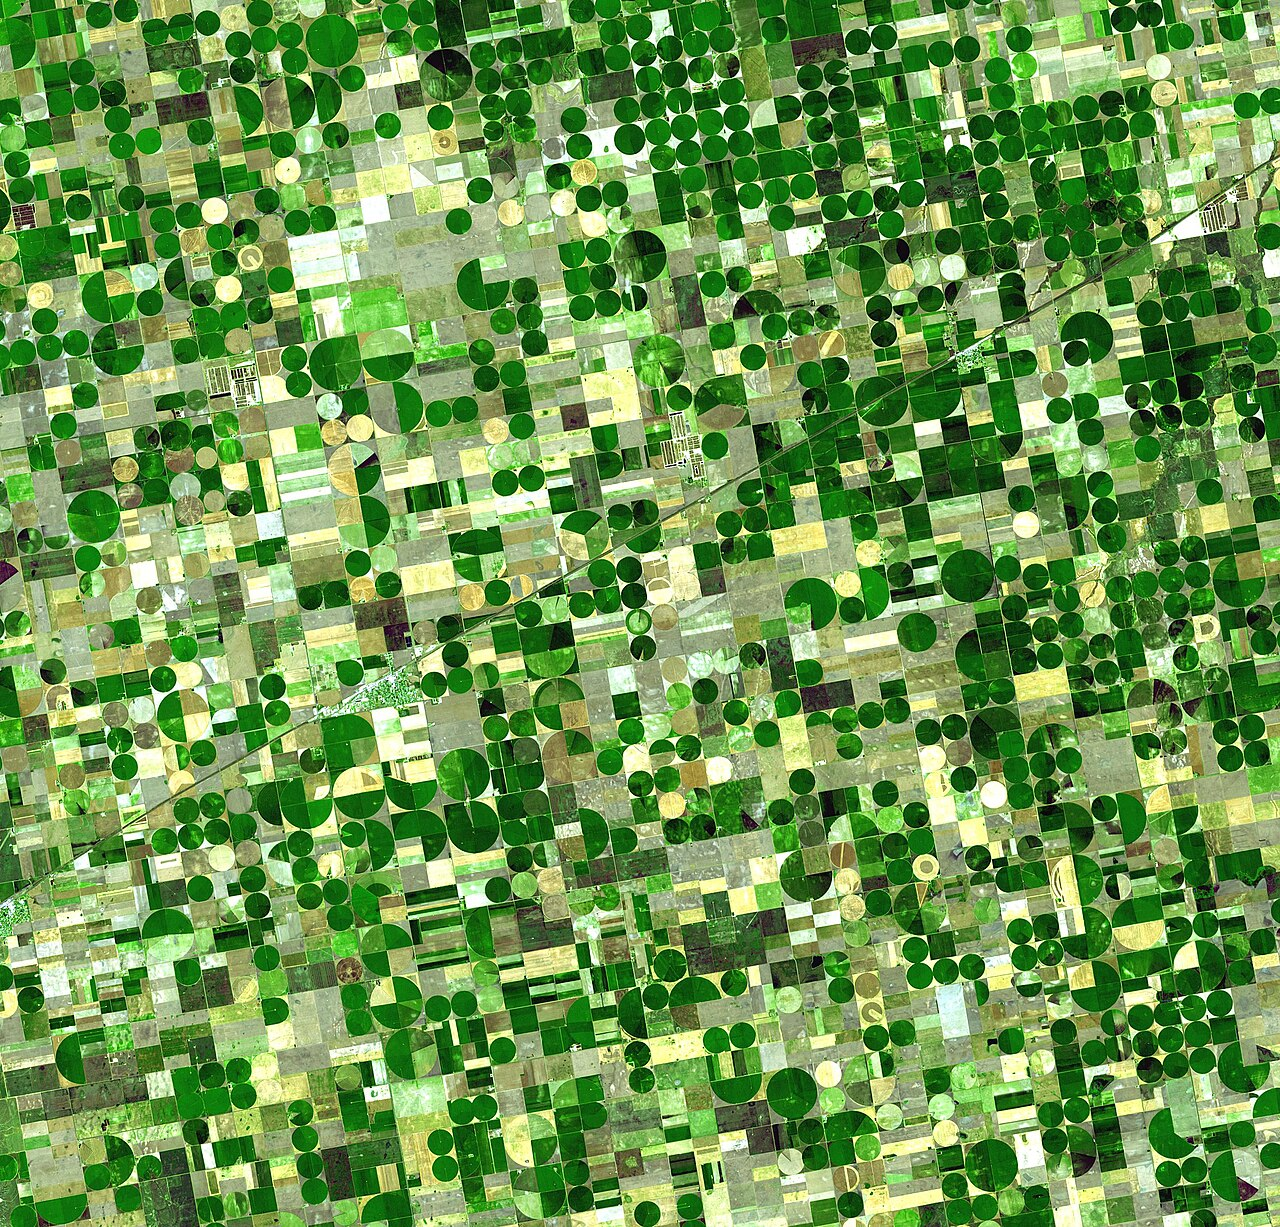
\includegraphics[width=0.5\linewidth]{images/book2/g10-nasa-kansas-center-pivot.jpg}

{\small Des champs irrigués près de Sublette, au Kansas, vus par
l'instrument ASTER du satellite Terra de la NASA en juin 2001 (environ
\qty{37}{km} de large). Chaque cercle est un champ arrosé par une longue
rampe d'arrosage qui tourne autour de son centre~; les cercles mesurent
\num{800} et \qty{1600}{m} de diamètre. Image~: NASA (domaine public).}
\end{omfigure}

Les eaux souterraines ne se voient pas depuis l'espace, mais on peut les
peser~: deux satellites qui volent l'un derrière l'autre perçoivent les
légères variations de l'attraction terrestre dues à la masse d'eau qui va et
vient sous eux, et cartographient où le \omterm{def:g10:freshwater-resources:stock}{stock} d'eau des terres augmente et
diminue d'un mois à l'autre.

\begin{omfigure}
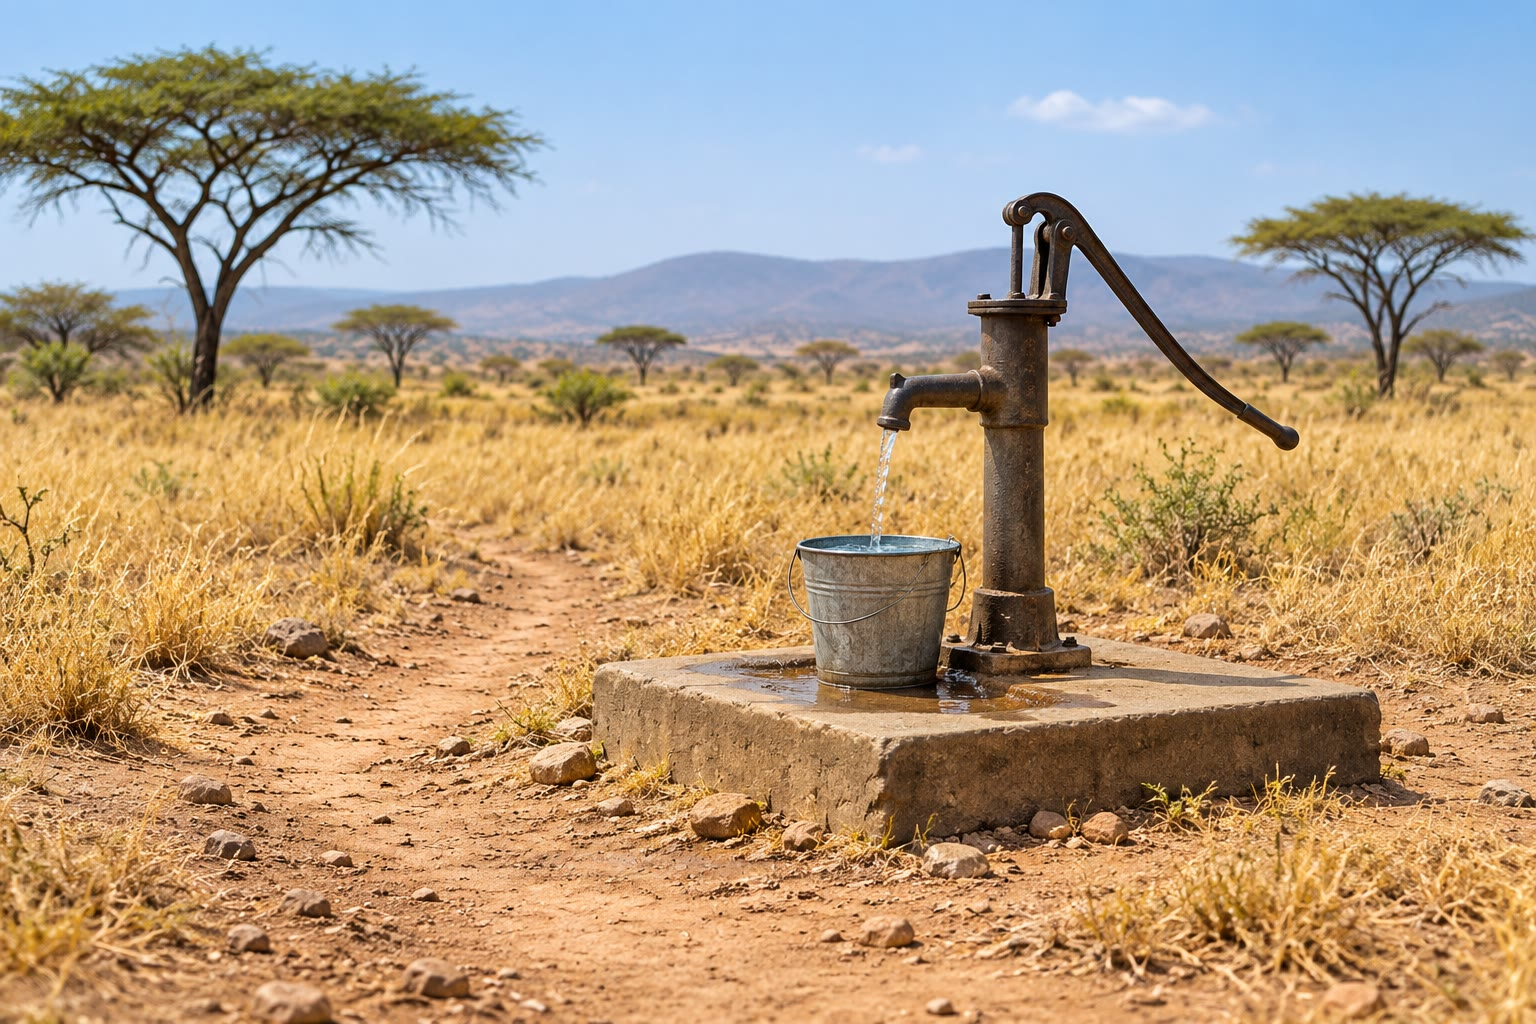
\includegraphics[width=0.55\linewidth]{images/book2/ai/g10-hand-pump-well.jpg}

{\small Une pompe à main sur un puits dans un paysage aride~: l'eau qu'on
tire ici vient du sous-sol, hors d'atteinte de la saison sèche.}
\end{omfigure}

\section{La surexploitation, un fait physique}

La mer d'Aral n'a pas d'exutoire~: l'eau de ses deux fleuves, l'Amou-Daria
et le Syr-Daria, n'en sort que par évaporation. En 1960, elle couvrait
\qty{68000}{km^2}, contenait \qty{1093}{km^3} et son eau renfermait
\qty{10}{g} de sel par litre. Cette année-là, l'évaporation a retiré
\qty{71.1}{km^3}, et la pluie tombée sur le lac a apporté \qty{9.4}{km^3}~:
pour garder son niveau, le lac avait besoin de
$71.1 - 9.4 = \qty{61.7}{km^3}$ par an venus de ses fleuves.
% ledger: gaybullaev:aral-1960, gaybullaev:aral-table

À partir des années 1960, les fleuves ont été détournés pour irriguer le
désert, et presque rien de leur eau n'atteignait plus le lac~: dans les
années 1970 et 1980, souvent moins de \qty{2}{km^3} par an. L'évaporation a
continué, et le lac a commencé à rétrécir. Son bilan fixe à quelle vitesse.
L'évaporation enlève une couche d'eau dont l'épaisseur dépend du climat,
ici environ un mètre par an
($71.1/68\,000 \approx \qty{0.00105}{km}$). Si l'apport cesse, le niveau
baisse chaque année d'à peu près autant, moins la pluie. À mesure que le lac
rétrécit, sa surface et donc son évaporation diminuent aussi, et la baisse
ralentit~; mais elle ne s'arrête que lorsque l'apport et l'évaporation
s'équilibrent de nouveau.
% ledger: gaybullaev:aral-table (values computed in figdata/grade-10/aral_sea.py)

\begin{omfigure}
\begin{tikzpicture}
\begin{axis}[omrecord, name=vol, width=0.46\linewidth, height=5.4cm, xmin=1955, xmax=2012, ymin=0, ymax=1200,
  xtick={1960,1980,2000}, xticklabel style={/pgf/number format/1000 sep={}}, scaled y ticks=false,
  ylabel={volume (\unit{km^3})}, xlabel={année}, tick label style={font=\small}, label style={font=\small},
  title={\small volume d'eau}]
\addplot[omDef, line width=1pt, mark=*, mark size=1.3pt] table[x=year, y=volume] {figdata/out/grade-10-aral_sea-record.dat};
\end{axis}
\begin{axis}[omrecord, at={(vol.east)}, anchor=west, xshift=1.4cm, width=0.46\linewidth, height=5.4cm,
  xmin=1955, xmax=2012, ymin=0, ymax=140, xtick={1960,1980,2000},
  xticklabel style={/pgf/number format/1000 sep={}},
  ylabel={salinité (\unit{g/L})}, xlabel={année}, tick label style={font=\small}, label style={font=\small},
  title={\small salinité}]
\addplot[omProp, line width=1pt, mark=*, mark size=1.3pt] table[x=year, y=salinity] {figdata/out/grade-10-aral_sea-record.dat};
\end{axis}
\end{tikzpicture}

{\small La mer d'Aral de 1960 à 2010~: le volume de son eau est tombé au
dixième, tandis que le sel laissé par l'évaporation est devenu treize fois
plus concentré. Données~: Gaybullaev et ses collègues (2012).}
\end{omfigure}
% ledger: gaybullaev:aral-table

En 2010, le lac contenait \qty{98}{km^3}, un dixième de son volume de 1960,
sur \qty{14280}{km^2}~; sa salinité avait atteint \qty{130}{g/L}, bien plus
que celle de l'océan. Son niveau avait baissé de plus de \qty{20}{m}. Des
poussières salées s'envolent du fond asséché. La cause n'a rien de caché~:
l'apport du lac a été coupé, son évaporation ne l'a pas été.
% ledger: gaybullaev:aral-table, gaybullaev:aral-1960, micklin:aral, nasa:aral

\section{Exercices}

\begin{exercise}[$\star$]\label{exo:g10:freshwater-resources:1}
Définir un \omterm{def:g10:freshwater-resources:stock}{stock}, un \omterm{def:g10:freshwater-resources:stock}{flux} et un \omterm{def:g10:freshwater-resources:residence-time}{temps de résidence}, et donner l'unité de
chacun.
\end{exercise}

\begin{exercise}[$\star$]\label{exo:g10:freshwater-resources:2}
D'après le tableau de l'eau du monde~: quelle part de toute l'eau est
douce~? Quelles parts de l'eau douce sont gelées, et souterraines~? Quel
réservoir en contient le moins~?
\end{exercise}

\begin{exercise}[$\star$]\label{exo:g10:freshwater-resources:3}
Définir l'\omterm{def:g10:freshwater-resources:renewable}{eau douce renouvelable} et l'\omterm{def:g10:freshwater-resources:fossil-groundwater}{eau souterraine fossile}. Pourquoi la
première est-elle un \omterm{def:g10:freshwater-resources:stock}{flux} et la seconde un \omterm{def:g10:freshwater-resources:stock}{stock}~?
\end{exercise}

\begin{exercise}[$\star$]\label{exo:g10:freshwater-resources:4}
Combien de fois plus d'eau les lacs d'eau douce du monde
(\num{91000}~\unit{km^3}) contiennent-ils que ses rivières
(\num{2120}~\unit{km^3})~?
\end{exercise}

\begin{exercise}[$\star$]\label{exo:g10:freshwater-resources:5}
Sur le graphique des \omterm{def:g10:freshwater-resources:residence-time}{temps de résidence}, quel réservoir renouvelle son eau
le plus vite, et lequel le plus lentement~? Combien de fois plus longtemps
l'eau reste-t-elle dans l'océan que dans l'air~?
\end{exercise}

\begin{exercise}[$\star\star$]\label{exo:g10:freshwater-resources:6}
L'atmosphère contient \num{12700}~\unit{km^3} d'eau. Calculer son \omterm{def:g10:freshwater-resources:residence-time}{temps de
résidence} à partir de l'évaporation qui y entre (\num{413000} depuis
l'océan et \num{73000}~\unit{km^3} depuis les terres chaque année), et
vérifier qu'il correspond au \omterm{def:g10:freshwater-resources:residence-time}{temps de résidence} calculé à partir des
précipitations qui en sortent.
\end{exercise}

\begin{exercise}[$\star\star$]\label{exo:g10:freshwater-resources:7}
L'océan contient \num{1335040}~milliers de~\unit{km^3} et perd
\num{413}~milliers de~\unit{km^3} par an par évaporation. Calculer son
\omterm{def:g10:freshwater-resources:residence-time}{temps de résidence}. Pourquoi est-il le même si on le calcule avec ce qui y
entre~?
\end{exercise}

\begin{exercise}[$\star\star$]\label{exo:g10:freshwater-resources:8}
À l'aide des \omterm{def:g10:freshwater-resources:stock}{flux} du cycle global de l'eau, écrire le bilan des terres~: ce
qui y tombe, ce qui retourne à l'air, ce qui ruisselle. Quelle part de la
pluie tombée sur les terres retourne à l'air~?
\end{exercise}

\begin{exercise}[$\star\star$]\label{exo:g10:freshwater-resources:9}
L'aquifère des Hautes Plaines a perdu environ \num{273.2}~millions
d'acres-pieds d'eau de 1950 environ à 2015 (\num{1}~acre-pied =
\qty{1233.5}{m^3}). Convertir ce volume en \unit{km^3} et le comparer au
volume de la mer d'Aral en 1987 (\qty{345.6}{km^3}).
\end{exercise}

\begin{exercise}[$\star\star$]\label{exo:g10:freshwater-resources:10}
Le niveau d'eau moyen de l'aquifère des Hautes Plaines a baissé de
\num{15.8}~pieds de 1950 environ à 2015 (\num{1}~pied = \qty{0.3048}{m}).
Combien cela fait-il en mètres, et en centimètres par an~?
\end{exercise}

\begin{exercise}[$\star\star$]\label{exo:g10:freshwater-resources:11}
Un aquifère contient \qty{2}{km^3} d'eau et reçoit une recharge de
\qty{0.01}{km^3} par an. Quel est le \omterm{def:g10:freshwater-resources:residence-time}{temps de résidence} de son eau~? Des
puits y pompent désormais \qty{0.05}{km^3} par an. On suppose que la
recharge continue et que les puits sont désormais la seule sortie de
l'eau~: combien de temps l'aquifère durera-t-il~?
\end{exercise}

\begin{exercise}[$\star\star\star$]\label{exo:g10:freshwater-resources:12}
Calculer le \omterm{def:g10:freshwater-resources:residence-time}{temps de résidence} de l'eau de la mer d'Aral en 1960
(\qty{1093}{km^3}, évaporation de \qty{71.1}{km^3} par an) et en 2010
(\qty{98.1}{km^3}, évaporation de \qty{11.4}{km^3} par an). Pourquoi son
évaporation a-t-elle diminué~?
\end{exercise}

\begin{exercise}[$\star\star\star$]\label{exo:g10:freshwater-resources:13}
Un lac sans exutoire couvre \qty{100}{km^2}. L'évaporation retire
\qty{1.2}{m} d'eau par an à sa surface, et la pluie en ajoute \qty{0.2}{m}.
\begin{enumerate}
  \item Quel apport, en \unit{km^3} par an, maintient son niveau
        constant~?
  \item L'apport est réduit de moitié. De combien le niveau baisse-t-il la
        première année~?
  \item Pourquoi la baisse ralentit-elle les années suivantes~?
\end{enumerate}
\end{exercise}

\begin{exercise}[$\star\star\star$]\label{exo:g10:freshwater-resources:14}
Dans un désert, la pluie recharge un aquifère de \qty{1}{mm} d'eau par an.
L'aquifère est épais de \qty{100}{m} et l'eau occupe \qty{20}{\percent} de
son volume. Combien de temps faudrait-il à la recharge pour le remplir~?
Comparer à l'âge de l'eau profonde de l'aquifère du Sahara.
\end{exercise}

\begin{exercise}[$\star\star\star$]\label{exo:g10:freshwater-resources:15}
L'aquifère des Hautes Plaines couvre environ \qty{453000}{km^2} et avait
perdu environ \qty{337}{km^3} d'eau en 2015. Quelle épaisseur d'eau,
répartie sur tout l'aquifère, cela représente-t-il~? Son niveau d'eau a
baissé de \qty{4.8}{m} en moyenne. Pourquoi la baisse du niveau d'eau
est-elle plus grande que l'épaisseur d'eau perdue~?
\end{exercise}

\section{Problème~: le bilan de la mer d'Aral}

\begin{problem}[{Problème du week-end --- à quelle vitesse un lac disparaît-il~?}]
\label{pb:g10:freshwater-resources:1}
% ledger: gaybullaev:aral-table, gaybullaev:aral-1960, micklin:aral (values computed in figdata/grade-10/aral_sea.py)
Le tableau donne le bilan de la mer d'Aral pour quatre années (volumes en
\unit{km^3}, salinité en grammes de sel par litre). En 1960, le lac
couvrait \qty{68000}{km^2}.
\begin{center}
\small
\begin{tabular}{|c|c|c|c|c|c|}
\hline
année & apport des fleuves & pluie sur le lac & évaporation & volume & salinité \\ \hline
1960 & 42.0 & 9.4 & 71.1 & 1093.0 & 10.0 \\ \hline
1984 & 0.3 & 3.5 & 47.9 & 502.7 & 21.9 \\ \hline
1987 & 1.0 & 6.2 & 36.8 & 345.6 & 25.0 \\ \hline
1989 & 3.1 & 5.3 & 35.3 & 327.2 & 30.0 \\ \hline
\end{tabular}

{\small Données~: Gaybullaev et ses collègues (2012).}
\end{center}

\medskip
\noindent\textbf{Partie I --- Le lac en 1960.}
\begin{enumerate}
  \item Quelle était la profondeur moyenne du lac en 1960~?
  \item Exprimer son volume en mètres cubes.
  \item Quelle masse de sel contenait-il, en tonnes~?
  \item Quel était le \omterm{def:g10:freshwater-resources:residence-time}{temps de résidence} de son eau, compté avec
        l'évaporation~?
  \item Pourquoi un lac sans exutoire ne peut-il perdre de l'eau que par
        évaporation (et par infiltration)~?
\end{enumerate}

\medskip
\noindent\textbf{Partie II --- Ce dont le lac a besoin.}
\begin{enumerate}[resume]
  \item Quelle épaisseur d'eau l'évaporation a-t-elle retirée du lac en
        1960, en mètres~?
  \item Quelle épaisseur la pluie a-t-elle ajoutée~?
  \item Quel apport des fleuves aurait exactement compensé l'évaporation
        et la pluie~?
  \item Les deux fleuves transportent en moyenne environ \qty{79}{km^3} et
        \qty{37}{km^3} par an au sortir des montagnes. Quelle part de ce
        total serait nécessaire au lac~?
\end{enumerate}

\medskip
\noindent\textbf{Partie III --- Le lac à la fin des années 1980.}
\begin{enumerate}[resume]
  \item Écrire le bilan de 1987~: entrées, sorties, variation nette.
  \item Entre 1984 et 1989, le volume est passé de \qty{502.7}{km^3} à
        \qty{327.2}{km^3}. Quelle a été la baisse moyenne par an~?
        Comparer avec le bilan de 1987.
  \item On suppose qu'un kilomètre carré de lac perd autant d'eau par
        évaporation qu'en 1960. Quelle était la surface du lac en 1987~?
  \item Quelle part de sa surface de 1960 cela représente-t-il~?
  \item Pourquoi l'évaporation était-elle tombée de \qty{71.1}{km^3} à
        \qty{36.8}{km^3}~?
  \item Quelle part de son volume de 1960 le lac contenait-il encore en
        1987~?
\end{enumerate}

\medskip
\noindent\textbf{Partie IV --- Le sel et le niveau.}
\begin{enumerate}[resume]
  \item Si tout le sel de 1960 était resté dans l'eau, quelle aurait été la
        salinité en 1987~?
  \item Le tableau donne \qty{25.0}{g/L}. Que suggère l'écart~?
  \item Sans aucun apport et sans aucune pluie, de combien le niveau
        baisserait-il chaque année~?
  \item En 1987, combien les fleuves et la pluie ont-ils ajouté, en
        épaisseur, sur la surface de la question 12~?
  \item De combien le niveau de la mer d'Aral a-t-il baissé en 1987~?
\end{enumerate}
\end{problem}
